\chapter{Anleitung für Docker starten}
\section{Docker starten}
\begin{enumerate}
    \item Verbinden mit HPC 
    \item Unter \textit{/mnt/data/outside-data/} Ordner mit Namen Projekt anlegen für Studierenden (\textit{mkdir \textless Projektname\textgreater}) 
    \item Studierenden privaten Key vom Nutzer \textit{docker\_user} geben
    \item Studierende kopiert Daten auf \textit{/mnt/data/outside-data/} $\rightarrow$ die folgenden Schritte beziehen sich auf ein Windows Betriebssystem, für Linuxsysteme sind die ähnlichen Schritte nur die Berechtigungsschritte werden per \textit{chown 700 \textless user\textgreater \textless key\textgreater}
    
    \begin{enumerate}
        \item Studierende speichert Private Key auf PC ab
        \item Verbindung des PCs mit Mosbach VPN (Lehre Netz)
        \item Rechtsklick auf private Key im File Explorer $\rightarrow$ Properties $\rightarrow$ Sicherheit $\rightarrow$ erweitert $\rightarrow$ sollte Berechtigung sehen wie in \autoref{fig:berecht_1}
        \item klicken auf Vererbung Deaktivieren
        \item Hinzufügen klicken $\rightarrow$ SYSTEM suchen $\rightarrow$ Lese- und Execute und Schreibrechte geben $\rightarrow$ Ok klicken
        \item Hinzufügen klicken $\rightarrow$ \textless eigenen Nutzer\textgreater  suchen $\rightarrow$ Lese- und Execute und Schreibrechte geben $\rightarrow$ Ok klicken
        \item danach sollte Berechtigung aussehen wie in \autoref{fig:berecht_2}
        \item Kommandozeile öffnen $\rightarrow$ wechseln in Directory wo Key legt
        \item Folgendes Kommando eingeben (alles eine Zeile)
        \begin{verbatim}
            scp -i <keyfile Name> -P 2022 <Pfad zu Datenablage>
            docker_user@193.197.11.229:/mnt/data/outside-data/
            <Name des Projektes>/  
        \end{verbatim}
        \item Information: \textless Pfad zu Datenablage\textgreater ist der Pfad zur Base Directory $\rightarrow$ alles darin wird rüberkopiert / \textless Name des Projektes\textgreater ist ein vorher angelegter Ordner, der den Namen des Projektes trägt, Password eingeben $\rightarrow$ wird von Herrn Müller übergeben
    \end{enumerate}
    \item Dockercontainer installieren $\rightarrow$ wenn YOLOv5 bitte unten den Anweisungen folgen
    \item Client schließen und laufen lassen
\end{enumerate}

\begin{figure}
    \centering
    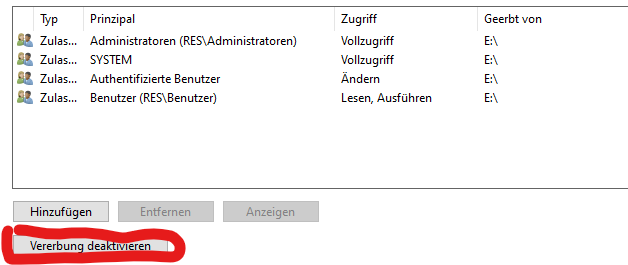
\includegraphics[width=8cm]{data/img/berechtigungen_1.png}
    \caption{Berechtigungen wie sie meistens voreingestellt sind durch Windows}
    \label{fig:berecht_1}
\end{figure}
\begin{figure}
    \centering
    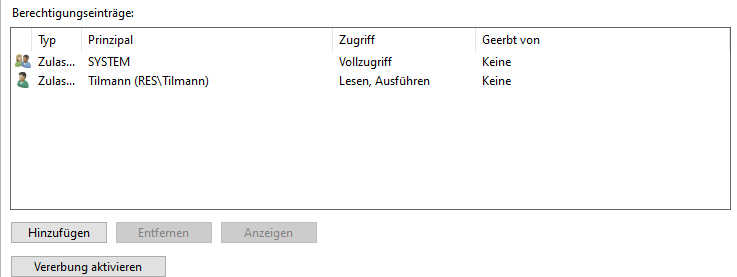
\includegraphics[width=8cm]{data/img/berechtigungen_2.png}
    \caption{Zielzustand Berechtigungen}
    \label{fig:berecht_2}
\end{figure}



\section{Docker YOLOv5 Container Setup und Vorbereitungen}

\textcolor{red}{\textbf{Wichtig:}} Die Umgebung mit YOLO und PyTorch ist schon aufgesetzt mit dem Dockercontainer der von Dockerhub gezogen wird. Insofern keine Änderungen am Algorithmus vorgenommen wurden, reicht dieser Container vollkommen aus und liefert alle nötigen Umgebungswerkzeuge


\begin{enumerate}
    \item Entsprechenden Dockercontainer Pullen per Kommando: \textit{docker pull ultralytics/yolov5:latest} 
    \item eingeben Kommando unten (alles eine Zeile)
    \begin{verbatim}
        docker run --ipc=host -it --gpus all --memory="<memory limit>"
        --cpus="<cpu limit>" -v 
        /mnt/data/outside-data/<projektname>/:/usr/src/datasets
        ultralytics/yolov5:latest
    \end{verbatim}
    \begin{itemize}
        \item \textless memory limit\textgreater  wird eingegeben wie viel GB der Container nutzen darf, dabei immer nur das Vorzeichen Gigabyte  $\rightarrow$ g / Megabyte $\rightarrow$ m
        \item \textless cpu limit\textgreater gibt an wie viele CPUs maximal genutzt werden dürfen vom Container als Gleitkommazahl $\rightarrow$ 2 CPUs entspräche 2.0
        \item sowohl die gpus flag, memory flag als auch cpu flag dürfen weg gelassen werden, dann läuft der Container auf der gesamten Hardware    
    \end{itemize}
    \item versichern Sie sich, dass die Daten unter \textit{/usr/src/datasets/} vorhanden sind
    \item geben sie \textit{exit} ein in die Kommandozeile 
    \item Eingeben des folgenden Kommandos:
    \begin{verbatim}
        docker start <cont_id>; docker exec <cont_id> <yolo_befehl> &
    \end{verbatim}
    \begin{itemize}
        \item  \textless cont\_id\textgreater  ist dabei die ID des jeweiligen Docker Containers
        \item \textless yolo\_befehl\textgreater  Befehl zum Ausführen des Detektionsskriptes siehe \autoref{sec:yolo_train}
    \end{itemize}
    \item Jetzt trainiert der Docker Container
\end{enumerate}

\subsection{YOLO Modell Trainieren}
\label{sec:yolo_train}
Um das Modell zu trainieren sollte in den Docker Container gewechselt werden und das Terminal geöffnet werden. Mit dem Kommando \textit{bash} wird in Bash gewechselt und es kann gesehen werden in welchem Ordner man sich befindet. 

Für das Training des Modells muss in das  Base Directory von dem YOLOv5 Repository gewechselt werden. Darin befindet sich die \textit{train.py} datei. Hierbei kann man das Training mit dem folgenden Befehl starten:
\begin{verbatim}
    python train.py --img <size_of_img> --batch <size_of_batches> --epochs <epochs>
    
    --data <data_path_to_yaml> --weights <weights> [--device <device_numbers> ]
\end{verbatim}
Die in eckickegen Klammern stehende Begriffe sollen nun nochmal erklärt werden:
\begin{itemize}
    \item \textless size\_of\_img\textgreater definiert die Breite des Bildes in Pixel. \textbf{Achtung:} Je höher der Pixelcount, desto höher der RAM / VRAM Verbrauch aber der Anstieg ist nicht linear, sondern Exponentiell
    \item \textless size\_of\_batch\textgreater gibt an wie viele Bilder in einem Durchgang (Epoche) analysiert werden soll. Diese kann per Hand vorgegeben werden, allerdings passiert es dann, dass aufgrund unzureichenden Videospeichers das Training abbricht. Für eine dynamische Anpassung des Videospeichers -1 eingeben. Allerdings kann es sein, dass dann alle Ressourcen genutzt werden.
    \item \textless epochs\textgreater gibt an wie oft trainiert wird. Für jede neue Epoche werden die nächsten Batch an Images analysiert bis alle Bilder analysiert sind und der Algorithmus beginnt wieder von vorne. Somit wird sichergestellt, dass bei einer hohen Anzahl an Bildern alle Bilder untersucht werden.
    \item \textless weights\textgreater Für das Training gibt es 5 verschiedene Gewichte: Nano, Small, Medium, Large und XLarge. Für die jeweiligen Gewichte muss folgendes eingegeben werden. Es sei zu beachten, dass mit zunehmender größe die Rechendauer und der Platz an benötigten Arbeitsspeicher massiv zunimmt.
    \begin{itemize}
        \item Nano $\rightarrow $ \textit{yolov5n.pt}
        \item Small $\rightarrow $ \textit{yolov5s.pt}
        \item Medium $\rightarrow $ \textit{yolov5m.pt}
        \item Large $\rightarrow $ \textit{yolov5l.pt}
        \item XLarge $\rightarrow $ \textit{yolov5x.pt}
    \end{itemize}
    \item \textless device\_numbers\textgreater dies ist auch für die Arbeit ein optionaler Parameter. Dieser gibt an welche GPUs genutzt werden sollen. Wird, das ausgelassen geht der Algorithmus von einer CPU Berechnung aus und nutzt den vorliegenden Arbeitsspeicher und die CPU. Damit GPU(s) genutzt werden können müssen die Nummern der GPUs angegeben werden. Diese wird durch das Betriebssystem bestimmt. Wenn nur eine GPU vorhanden ist, ist dies i.d.R. 0. Damit wird der komplette VRAM der GPU genutzt. Voraussetzung dafür ist es, dass das NVIDIA CUDA Toolkit installiert ist und der GPU für den Docker freigeschaltet ist, was jedoch der default ist. Für mehrere GPUs einfach mit Kommata die GPUs auflisten. Für mehr Informationen \textit{\href{https://github.com/ultralytics/yolov5/issues/475}{hier klicken}}.
\end{itemize}

\section{Den Docker Contaioner anschauen}
Dieser Abschnitt befasst sich damit wie man während des Laufes den Docker Container betreten kann ohne, dass der Trainingsprozess stoppt
\begin{enumerate}
    \item Docker Container anzeigen lassen mit \textit{docker ps}
    \item Konsole des Dockercontainer verbinden \textit{docker attach \textless cont\_id\textgreater} $\rightarrow$ damit wird die Konsolenausgabe des Dockercontainers mit der eigenen verbunden
    \item bei Verlassen erst \textit{Strg + P} und anschließend \textit{Strg + Q} drücken 
\end{enumerate}

\section{Docker Container stoppen und löschen}
Zum Stoppen des Containers kann der folgende Befehl gesetzt werden:
\begin{verbatim}
    docker stop <container_name>
\end{verbatim}
Der \textless container\_name\textgreater kann durch den Befehl \textit{docker ps} angezeigt werden. Dabei wird in der letzten Spalte der Containername angezeigt und in der ersten Spalte die id. \textit{docker stop} nutzt die ID des Docker Containers.

Mit dem Befehl \textit{docker rm \textless container\_id\textgreater} kann dann der Container gelöscht werden 